\chapter[Анализ стран: возраст, формы правления и этнохоронимы]{Анализ трёх аспектов современных стран по Викиданным:\\возраст стран, популярные формы правления и этнохоронимы}
\label{ch:country}

Глава посвящена исследованию стран на основе Викиданных. 
С помощью SPARQL-запросов, вычисляемых на объектах <<страна>>, получены: 
список современных стран, перечень всех стран, упорядоченных по дате создания, 
список этнохоронимов стран. 
Построены пузырьковая диаграмма с формами правления стран, 
граф соседних стран и карта соседних стран России. 
Выполнена оценка Викиданных по количеству исторических и~современных стран, 
по количеству заполненных этнохоронимов у~стран. 
%%%%%%%%%%%%%%%%%%%%%%%%%%%%%%%%%%%%%%%%%%%%%%%%%%%%%%%


\begin{marginfigure}[7\baselineskip]
%\setlength{\fboxsep}{0pt}%
%\setlength{\fboxrule}{1pt}%
%\fcolorbox{gray}{gray}{
    \includegraphics[width=0.8\linewidth]{chapter/country/ProWD_country.png}
    \caption[Степень заполненности свойств стран на Викиданных]%
	{%
Высокая степень заполнения по числу свойств объекта Викиданных \href{https://www.wikidata.org/wiki/Q6256}{страна (Q6256)}.  Данные получены с помощью сервиса \href{https://prowd.id/dashboards/86b6f91a8131/profile}{ProWD.id}, 2020 год. \emph{Коэффициент Джини равен 0.091.}
	}%
	\label{fig:ProWD_country}%
\end{marginfigure}


\section{Список стран и степень полноты информации ряда стран}

Построим список всех стран на английском и русском языках (листинг~\ref{lst:country}).

\begin{lstlisting}[ language=SPARQL, 
    caption={\href{https://w.wiki/k6L}{Экземпляры объекта <<страна>>}\protect\footnotemark},
    label=lst:country, 
    numbers=none,
]
#List of countries in English and Russian
SELECT ?country ?label_en ?label_ru WHERE
{
		?country wdt:P31 wd:Q6256. # instance of country
		?country rdfs:label ?label_en filter (lang(?label_en) = "en").
		?country rdfs:label ?label_ru filter (lang(?label_ru) = "ru").
}
\end{lstlisting}
\footnotetext[1][0cm]{Получено: 205 стран на 2017 год и 175 стран на 2020 год. Ссылка на SPARQL-запрос: \href{https://w.wiki/k6L}{https://w.wiki/k6L}}

%По степени заполненности свойств на Викиданнных можно различать <<полные>> и  <<пустые>> страны. 
%
%Примерами наиболее полных и проработанных стран на Викиданных по данным ProWD\autocite{prowd_balakireva} являются: \wdqName{Израиль}{801} (127 свойств), \wdqName{Франция}{142} (126 свойств), \wdqName{Соединённые Штаты Америки}{30} (124 свойства).
%
%Наименьшее количество свойств у \wdqName{Соединённых провинций Центральной Америки}{8842993} (3 свойства) и \wdqName{Джалаириды}{8842993} (9 свойств).



%%%%%%%%%%%%%%%%%%%%%%%%%%%%%%%%%%%%%%%%%%%%%%%%%%%%%%%
\section{Возраст стран и почему Россия бывает не страной? О конструкции p:/ps:}
\label{ch:RussiaNotCountryPPS}


%%%%%%%%%%%%%%%% Упражнение 2 %%%%%%%%%%%%%%%%
\marginnote{
%	Какое количество административных единиц имеют следующие страны:
	У \href{https://w.wiki/mzN}{Латвии} их 119, у \href{https://w.wiki/mzP}{Таиланда} 77, у \href{https://w.wiki/mzR}{Дании} 5, а у \href{https://w.wiki/myt}{России} 81. О количестве чего идет речь?
	\begin{itemize}
		\item Количество городов с населением более миллиона человек?
		\item Количество высших учебных заведений?
		\item Количество административных единиц?
		\item Количество официальных языков?
	\end{itemize}
	См. ответ~\ref{answer:administrative_territorial} на с.~\pageref{answer:administrative_territorial}.
}

Построим список стран, отсортированных по дате основания страны, то есть по первому упоминанию о стране (листинг~\ref{lst:age_of_country}).

\begin{lstlisting}[ language=SPARQL, 
caption={\href{https://w.wiki/suP}{Даты основания стран}\protect\footnotemark},
label=lst:age_of_country, 
]
# List of countries sorted by inception 
SELECT ?country ?countryLabel ?inception
WHERE
{
	?country wdt:P31 wd:Q6256.    # instance of country
	?country wdt:P571 ?inception. # the first mention
	SERVICE wikibase:label { bd:serviceParam wikibase:language "ru" }
}
ORDER BY (?inception)
\end{lstlisting}

\footnotetext{Получено  112 стран на 2017 год и 199 стран на 2020. Ссылка на SPARQL-запрос: \href{https://w.wiki/suP}{https://w.wiki/suP}}

В результате выполнения запроса (листинг~\ref{lst:age_of_country}) 
получен скромный список стран, включающий на 2020 год всего 199 стран. 
На примере России разберёмся, в чём здесь дело. 
Объект \wdqName{Россия}{159} в~поле \lstinline|instance of| содержит не одно, а восемь значений, в том числе \wdqName{country}{6256}.
%
\marginnote{%
На странице Викиданных \href{https://w.wiki/LX}{``Request a query''} одни редакторы задают вопросы, как написать тот или иной скрипт, а другие редакторы отвечают. Пользуйтесь этим форумом.
}

Решение и ответ на этот вопрос были найдены на странице ``Wikidata: Request a query'', а именно в разделе доступном по ссылке \href{https://w.wiki/tLm}{https://w.wiki/tLm}.

Дело в том, что конструкция wdt позволяет находить только истинные значения. 
Для~России предпочтительным ответом (англ. preferred value) 
в поле \lstinline|instance of| указано <<суверенное государство>>, а не <<страна>>. 
Чтобы проверить все варианты, представленные в поле \lstinline|instance of| России, 
нужно использовать конструкцию \lstinline|p:/ps:|.

Таким образом, запрос~\ref{lst:list_of_country_instance_of} 
позволяет получить больше стран, отсортированных по дате создания. 
В 2020 году было получено 235~стран, в 2022~--- 246~стран.


\newpage
\begin{lstlisting}[ language=SPARQL, 
caption={\href{https://w.wiki/5BCN}{Список стран, отсортированных по дате основания}\protect\footnotemark},
label=lst:list_of_country_instance_of, 
]
# List of countries sorted by inception date
SELECT ?country ?countryLabel (MIN(?year) AS ?min_year) WHERE
{
    ?country p:P31  [ps:P31 wd:Q6256];      # instance of a country 
             p:P571 [ps:P571 ?inception].   # all inception dates
    BIND(YEAR(?inception) AS ?year)
    SERVICE wikibase:label { bd:serviceParam wikibase:language "ru" }
}
GROUP BY ?country ?countryLabel
ORDER BY ?min_year
\end{lstlisting}
\footnotetext{Получено 235 стран в~2020 году, 246~стран в~2022~году. Ссылка на SPARQL-запрос: \href{https://w.wiki/5BCN}{https://w.wiki/5BCN}}

Чтобы убрать из этого списка уже не существующие страны, 
то есть экземпляры объекта \wdqName{historical country}{3024240}, 
используем оператор \lstinline|MINUS|. 
С помощью запроса~\ref{lst:list_of_country_instance_of_} получили список действующих, 
то есть не исторических, стран с известной датой основания.

\begin{lstlisting}[ language=SPARQL, 
caption={\href{https://w.wiki/5BCP}{Список стран, отсортированных по дате основания, не включающий исторические страны}\protect\footnotemark},
label=lst:list_of_country_instance_of_, 
]
# List of countries sorted by inception date without historical countries
SELECT ?country ?countryLabel (MIN(?year) AS ?min_year) WHERE
{
	?country p:P31 [ps:P31 wd:Q6256].               # instance of a country 
	MINUS {?country p:P31 [ps:P31 wd:Q3024240]}.    # except historical countries
	?country p:P571 [ps:P571 ?inception].           # all inception dates
	BIND(YEAR(?inception) AS ?year)
	SERVICE wikibase:label { bd:serviceParam wikibase:language "ru" }
}
GROUP BY ?country ?countryLabel
ORDER BY ?min_year
\end{lstlisting}

\footnotetext{Получено 211 стран в 2020 году и 212 в 2022 году. Ссылка на SPARQL-запрос: \href{https://w.wiki/5BCP}{https://w.wiki/5BCP}}

Например, первое упоминание о~\wdqName{Франции}{142} было в~463~году, о~\wdqName{России}{159}~--- в~862~году, о~\wdqName{Республике~Косово}{1246}~--- в~2008~году, о~\wdqName{Южном~Судане}{958}~--- в~2011~году. 
Наибольшее количество стран появилось в 1960 году (16 стран), 
в 1991 году (15 стран), в~1962~году (6~стран) и в~1821~году (6~стран).


\newpage
Выведем список стран с пустым свойством <<дата основания>> (листинг~\ref{lst:without_inception}). 
Такие некомплектные объекты Викиданных могли быть созданы по ошибке или могут содержать какие-то дефекты. 
Можно посмотреть историю правок объекта и обратиться с~вопросом к~редакторам этой статьи. 
Подробнее о том, что такое <<история правок>> в~вики-проектах 
и как с ней работать см. в~учебнике\autocite{Krizhanovsky2015}.

\begin{lstlisting}[ language=SPARQL, 
    caption={\href{https://w.wiki/k6q}{Страны с незаполненной датой основания}\protect\footnotemark},
    label=lst:without_inception,
    numbers=none,
]
#List of `instances of` "countries without a inception" 
SELECT ?country ?countryLabel WHERE
{
    ?country wdt:P31 wd:Q6256.      # instance of country
    MINUS { ?country wdt:P571 [] }. # inception of country is empty
    SERVICE wikibase:label { bd:serviceParam wikibase:language "ru" }
}
\end{lstlisting}
\footnotetext{Получено  100 стран на 2017 год и 7 стран на 2020 год. Ссылка на SPARQL-запрос: \href{https://w.wiki/k6q}{https://w.wiki/k6q}}




\subsection{Объём Викиданных по современным и историческим странам}

Проанализируем полноту Викиданных на примере исторических и~современных стран. 
По данным <<Общероссийского классификатора стран мира>>\autocite{oksm} на Земле существует 251~страна.
Отдельного анализа заслуживают древние, уже не существующие государства, например, \wdqName{Ассирия}{41137}. 
Объекты таких стран на Викиданных являются экземплярами не~объекта ``country'', 
а  ``historical country'' (историческая страна). 

С помощью скрипта~\ref{lst:List_of_historical_countries} построим список исторических государств. 
Таких бывших государств на 2020 год оказалось три тысячи, что на порядок больше числа современных государств.
%
%%%%%%%%%%%%%%%% Упражнение 2 %%%%%%%%%%%%%%%%
\marginnote{%
%	Какое количество административных единиц имеют следующие страны:
Напишите запрос, чтобы найти государства, существовавшие дольше всех.\\
См. ответ~\ref{answer:old_countries} на с.~\pageref{answer:old_countries}.
}


\begin{lstlisting}[ language=SPARQL, 
    caption={\href{https://w.wiki/tQN}{Список исторических стран}\protect\footnotemark},
    label=lst:List_of_historical_countries, 
    numbers=none,
]
# List of historical countries
SELECT ?country ?countryLabel WHERE
{
    ?country p:P31 [ps:P31 wd:Q3024240].    # instance of a historical country 
    SERVICE wikibase:label { bd:serviceParam wikibase:language "ru,en"} 
}
\end{lstlisting}
\footnotetext{Получено \num{3026} стран на 2020 год. Ссылка на SPARQL-запрос: \href{https://w.wiki/tQN}{https://w.wiki/tQN}}

%Отметим, что количество бывших стран (165 на 2020 год) меньше существующих ныне стран.

По данным статей <<Список государств>>\autocite{list_of_sovereign_states} Русской Википедии 
и статьи ``List of sovereign states''\autocite{list_of_sovereign_states_en} Английской Википедии существует 208 стран.

%%%%%%%%%%%%%%%% Упражнение 3 %%%%%%%%%%%%%%%%
\marginnote{%
Определите по флагам страны Азии и перечислите их в порядке возрастания плотности населения. 
См. ответ~\ref{answer:population_density} на с.~\pageref{answer:population_density}.
}
\begin{marginfigure}[0.0cm]
    \centering
        \includegraphics[width=3cm]{./chapter/country/256px-Flag_of_South_Korea.png}
	\caption{Флаг первой страны.}%
	\label{fig:flag_kor}%
\end{marginfigure}
\begin{marginfigure}[0.0cm]
    \centering
	    \setlength{\fboxsep}{0pt}%
	    \setlength{\fboxrule}{1pt}%
	    \fcolorbox{gray}{gray}{
        \includegraphics[width=3cm]{./chapter/country/256px-Flag_of_Singapore.png}}
	\caption{Флаг второй страны.}%
	\label{fig:flag_singapore}%
\end{marginfigure}


У экземпляров объекта <<\href{https://www.wikidata.org/wiki/Q6256}{страна}>> обычно заполнено свойство \href{https://www.wikidata.org/wiki/Property:P571}{inception (P571)}, то есть дата основания. Однако не всегда точно можно  указать дату основания страны по разным причинам: отсутствие, недостаток или противоречие письменных источников. Например, основание Древнерусского государства связывают с призванием варяжского князя Рюрика в 862 году, но точной даты нет (объект \wdqName{Россия}{159}). 
Некоторым современным странам предшествовал ряд исторических событий, 
и дату какого из них считать за дату создания современной страны~--- это вопрос открытый. 
Например, датой основания \wdqName{Монголии}{711} принято считать 29 декабря 1911 года, 
когда произошло провозглашение независимости от~Китая. 
Хотя в истории Монголия появляется со времён деятельности Чингисхана, 
который кратковременно в начале XIII 
%\MakeUppercase{\romannumeral13} 
века объединил под своей властью большую часть Евразии.



%%%%%%%%%%%%%%%%%%%%%%%%%%%%%%%%%%%%%%%%%%%%%%%%%%%%%%%
\section{Этнохоронимы стран на русском языке}

\begin{marginfigure}[0.0cm]
    \centering
%		\setlength{\fboxsep}{0pt}%
%		\setlength{\fboxrule}{1pt}%
%		\fcolorbox{gray}{gray}{
    \includegraphics[width=3cm]{./chapter/country/256px-Flag_of_Israel.png}
	\caption{Флаг третьей страны.}%
	\label{fig:flag_israel}%
\end{marginfigure}
\begin{marginfigure}[0.0cm]
    \centering
		\includegraphics[width=3cm]{./chapter/country/256px-Flag_of_Mongolia.png}
	\caption{Флаг четвертой страны.}%
	\label{fig:flag_mongolia}%
\end{marginfigure}
%\marginnote{
%	См. ответ~\ref{answer:population_density} на с.~\pageref{answer:population_density}.
%}

Этнохороним~--- это название жителей определённой местности, соотнесённое с топонимом. 
Например, этнохронимами для России будут россияне, россиянин, россиянка, 
для~Чехии~--- чехи, чех, чешка.

Помимо географического фактора, новые лексемы, используемые для определения происхождения либо принадлежности, происходят так же от этнических, политических, религиозных характеристик людей\autocite{Zhuravleva2012}. 

Этнохоронимы могут определяться названиями разных объектов земной поверхности: гор, островов, континентов. Так же обозначение места происхождения людей может зависеть от политико-административного деления. Например, для обозначения гражданства: Тайланд~--- тайландцы, Канада~--- канадцы. Внутригосударственное деление также может породить новые наименования, Крым~--- крымчане.



\newpage
Построим список стран, у которых есть этнохоронимы на русском языке (листинг~\ref{lst:demonym}).


\begin{lstlisting}[ language=SPARQL, 
caption={\href{https://w.wiki/tec}{Список стран с этнохоронимами на русском языке}\protect\footnotemark},
label=lst:demonym, 
]
# List of countries with demonyms in Russian
SELECT ?country ?countryLabel WHERE
{
	?country p:P31 [ps:P31 wd:Q6256]. # instance of a country
	?country wdt:P1549 ?demonym .     # has demonym
	FILTER((LANG(?demonym)) = "ru")
	SERVICE wikibase:label { bd:serviceParam wikibase:language "ru" }
}
GROUP BY ?country ?countryLabel
\end{lstlisting}
\footnotetext{Получено 28 стран на 2017 год и 131~--- на 2021 год. Ссылка на~SPARQL-запрос: \href{https://w.wiki/tec}{https://w.wiki/tec}}





\subsection{Cписок этнохоронимов стран}

%%%%%%%%%%%%%%%% Упражнение 4 %%%%%%%%%%%%%%%%
\marginnote{%
Какие из языков \href{https://w.wiki/myv}{абазинский}, \href{https://w.wiki/myx}{мокшанский}, \href{https://w.wiki/myy}{эрзянский}, \href{https://w.wiki/myz}{белорусский} являются официальными в \href{https://w.wiki/myt}{России}?%
См. ответ~\ref{answer:official_language} на с.~\pageref{answer:official_language}.
}

Построим список этнохоронимов стран на русском языке (листинг~\ref{lst:list_demonym}).

\index{SPARQL!FILTER!Cписок этнохоронимов}
\begin{lstlisting}[ language=SPARQL, 
caption={\href{https://w.wiki/teg}{Cписок этнохоронимов}\protect\footnotemark},
label=lst:list_demonym, 
]
# List of demonyms of countries in Russian
SELECT ?country ?countryLabel ?demonym
WHERE
{
	?country p:P31 [ps:P31 wd:Q6256]. # instance of a country
	?country wdt:P1549 ?demonym .     # has demonym
	FILTER((LANG(?demonym)) = "ru")
	SERVICE wikibase:label { bd:serviceParam wikibase:language "ru" }
}
\end{lstlisting}

\footnotetext{Получено  83 этнохоронима на 2017 год и 296 этнохоронимов на 2021 год. Ссылка на SPARQL-запрос: \href{https://w.wiki/teg}{https://w.wiki/teg}}




\newpage
\subsection{Страны с незаполненными этнохоронимами}

Построим список стран, у которых нет этнохоронимов на русском языке (листинг~\ref{lst:without_demonym}). 
Этот список может быть полезен редактору для добавления этнохоронимов. 


\index{SPARQL!FILTER!Страны с незаполненными этнохоронимами на русском языке}
\index{SPARQL!MINUS!Страны с незаполненными этнохоронимами на русском языке}
\begin{lstlisting}[ language=SPARQL, 
caption={\href{https://w.wiki/teo}{Страны с незаполненными этнохоронимами на русском языке}\protect\footnotemark},
label=lst:without_demonym, 
]
#List of countries without demonyms in Russian
SELECT ?country ?countryLabel WHERE
{
	?country p:P31 [ps:P31 wd:Q6256].       # instance of a country
	MINUS { ?country wdt:P1549 ?demonym.    # without demonyms
        FILTER((LANG(?demonym)) = "ru")     # in Russian
	}
	SERVICE wikibase:label { bd:serviceParam wikibase:language "ru" }
}
GROUP BY ?country ?countryLabel
\end{lstlisting}
\footnotetext{Получено 170 стран на 2017 год и 105 стран на 2021 год. Ссылка на~SPARQL-запрос: \href{https://w.wiki/teo}{https://w.wiki/teo}}

Благодаря конструкции MINUS в~строках 5--7 запроса~\ref{lst:without_demonym} 
в итоговый список не попали страны, имеющие этнохоронимы на русском языке.





\subsection{Количество заполненных этнохоронимов у стран}
%
\begin{marginfigure}[-5\baselineskip]
\begin{lstlisting}[ 
    language=SPARQL, 
    caption={\href{https://w.wiki/5BX5}{Список стран, упорядоченный по количеству заполненных этнохоронимов}},%\protect\footnotemark},
    label=lst:count_demonym, 
    numbers=none,
]
# List of countries ordered by number of demonyms
SELECT  ?country ?countryLabel (COUNT(*) AS ?demonyms) 
WHERE
{
  ?country p:P31 [ps:P31 wd:Q6256]; # instance of a country
           p:P1549 [ps:P1549 []].   # has demonym
  SERVICE wikibase:label {bd:serviceParam 
                          wikibase:language "ru"}
}
GROUP BY ?country ?countryLabel 
ORDER BY DESC(?demonyms)
\end{lstlisting}
%\footnotetext{Получено 199 стран на 2017 год и 215 стран на 2021 год. Ссылка на SPARQL-запрос: \href{https://w.wiki/5BX5}{https://w.wiki/5BX5}}
Получено 199 стран на 2017 год и 215 стран на 2021 год. Ссылка на SPARQL-запрос: \href{https://w.wiki/5BX5}{https://w.wiki/5BX5}
\end{marginfigure}%


У одной страны может быть от нуля, если данные не заполнены, до трёх-четырёх этнохоронимов. 
Например, у Турции есть три названия жителей: турок, тарчанка, турки, 
у~Эфиопии~--- четыре: эфиоп, эфиопка, эфиопы, эфиопки.

Получим список стран, упорядоченный по количеству заполненных в Викиданных этнохоронимов 
на разных языках (листинг~\ref{lst:count_demonym}). 
По данным на 2017 год больше всего этнохоронимов у~Соединённых Штатов Америки (41 этнохороним), 
затем идут Великобритания (40), 
Германия (40) и Канада (36). 
В~2021~году лидером стала Германия с 64 этнохоронимами, 
затем идут Россия~(61 этнохороним), Канада~(60) и~США~(60). 
Таким образом, с 2017 по 2021 год добавилось примерно по~20~этнохоронимов на одну страну.


%%%%%%%%%%%%%%%%%%%%%%%%%%%%%%%%%%%%%%%%%%%%%%%%%%%%%%%
\section{Формы правления стран}

Построим пузырьковую диаграмму форм правления стран (листинг~\ref{lst:form_of_government}), где размер пузырка будет соответствовать числу стран с той или иной формой правления.


%%%%%%%%%%%%%%%% Упражнение 4 (TODO: добавить ответ) %%%%%%%%%%%%%%%%
\marginnote[2cm]{%
Какая строка в запросе~\ref{lst:form_of_government} является лишней? То есть её можно удалить и~результат не~изменится. 
Речь не о первой строке с комментарием.%
}
\index{График!BubbleChart!Число стран с разными формами правления}
\begin{lstlisting}[ language=SPARQL, 
caption={\href{https://w.wiki/5BVh}{Число стран с разными формами правления}\protect\footnotemark},
label=lst:form_of_government, 
]
# Forms of government ordered by number of countries
#defaultView:BubbleChart
SELECT ?bfog ?form (COUNT(*) AS ?countries)
WHERE 
{
  ?country p:P31 [ps:P31 wd:Q6256]; # instance of a country
           p:P122 [ps:P122 ?bfog].  # basic form of government
  OPTIONAL {
    ?bfog rdfs:label ?form
	FILTER (LANG(?form) = "ru")
  }
  SERVICE wikibase:label { bd:serviceParam wikibase:language "ru"}
}
GROUP BY ?bfog ?form
ORDER BY DESC(?countries) ASC(?form)
\end{lstlisting}
\footnotetext{Получено 30 форм правления на 2017 год и 41 форма правления на 2021 год. Ссылка на SPARQL-запрос: \href{https://w.wiki/5BVh}{https://w.wiki/5BVh}}



Переменная \lstinline|bfog| (сокращение от ``basic form of government'') содержит форму правления, например, <<республику>>. 
Последняя сточка в листинге~\ref{lst:form_of_government} содержит команды упорядочения 
сначала по убыванию (DESC) и затем по возрастанию (ASC). 
Таким образом, формы правления сначала сортируются по числу стран \lstinline|?countries|. 
Затем, если стран оказалось поровну, то формы правления сортируются лексикографически\footnote{%
%
Лексикографический (словарный) порядок~--- это способ упорядочивания и сортировки слов, 
который обычно используется в словарях, энциклопедиях и алфавитных указателях. 
Например, А < АА < ААА < ААБ < ААВ < АБ < Б < … < ЯЯЯ.%
}.

В результате выполнения запроса мы получаем пузырьковую диаграмму с наиболее распространенными формами правления в странах на 2017 год (рис.~\ref{fig:bubble_chart_forms_of_government_countries_2017}) и на 2020 год (рис.~\ref{fig:bubble_chart_forms_of_government_countries_2020}).
Видим, что за период с 2017 по 2020 год 
форма правления <<республика>> стала более <<популярной>> 
(размер кружка относительно других стал больше). 
Значительно уменьшилось количество стран, имеющих форму  <<смешанная республика>>.


\begin{fullwidth}
\noindent\begin{minipage}[]{.484\linewidth}
    \centering
	    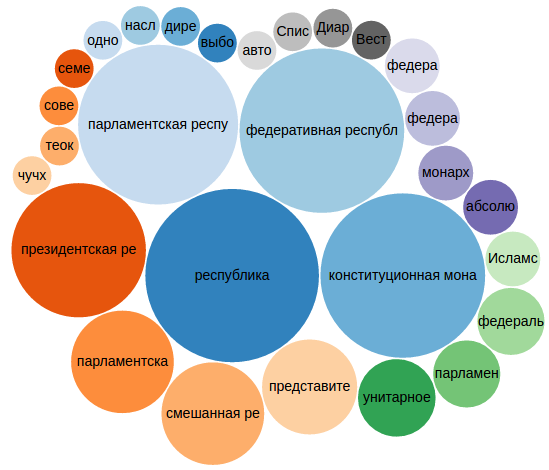
\includegraphics[width=0.94\linewidth]{./chapter/country/Bubble_chart_forms_of_government_countries_according_to_Wikidata.png}
        \caption{Пузырьковая диаграмма форм правления стран, 2017 год. По данным на 2017 год основные формы правления стран: республика (в 20 странах), конституционная монархия (в 18 странах), федеративная республика (18), парламентская республика (17) и президентская республика (12).} 
	    \label{fig:bubble_chart_forms_of_government_countries_2017}%
\end{minipage}%
%just a break for lines between two columns of listings
\hfill
\begin{minipage}[]{.46\linewidth}
    \centering
	\includegraphics[width=0.95\linewidth]{./chapter/country/Bubble_chart_forms_of_government_countries_according_to_Wikidata_2020.png}
    \caption{Пузырьковая диаграмма форм правления стран, 2020 год.
	\\
	По данным на 2020 год  основные формы правления стран: республика (в~41~стране), конституционная монархия (32), федеративная республика (19), парламентская республика (22) и президентская республика (14).} 
	\label{fig:bubble_chart_forms_of_government_countries_2020}%
\end{minipage}
\end{fullwidth}%


%\begin{figure}
%		\setlength{\fboxsep}{0pt}%
%		\setlength{\fboxrule}{1pt}%
%		\fcolorbox{gray}{gray}{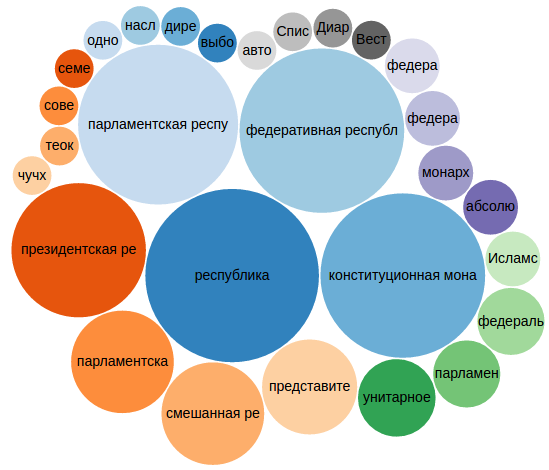
\includegraphics[width=\linewidth]{./chapter/country/Bubble_chart_forms_of_government_countries_according_to_Wikidata.png}}%
%	\caption
%	[Пузырьковая диаграмма форм правления стран, 2017 год.]
%	{Пузырьковая диаграмма форм правления стран, 2017 год.
%		\\			
%		По данным на 2017 год основные формы правления стран: республика (в 20 странах), конституционная монархия (в 18 странах), федеративная республика (18), парламентская республика (17) и президентская республика (12).}%
%	\label{fig:bubble_chart_forms_of_government_countries_2017}%
%\end{figure}

%\begin{figure}
%		\setlength{\fboxsep}{0pt}%
%		\setlength{\fboxrule}{1pt}%
%		\fcolorbox{gray}{gray}{\includegraphics[width=\linewidth]{./chapter/country/Bubble_chart_forms_of_government_countries_according_to_Wikidata_2020.png}}%
%	\caption
%	[Пузырьковая диаграмма форм правления стран, 2020 год.]
%	{Пузырьковая диаграмма форм правления стран, 2020 год.
%	\\
%	По данным на 2020 год  основные формы правления стран: республика (в 41 стране), конституционная монархия (32), федеративная республика (19), парламентская республика (22) и президентская республика (14).
%}%
%	\label{fig:bubble_chart_forms_of_government_countries_2020}%
%\end{figure}




\newpage
%%%%%%%%%%%%%%%%%%%%%%%%%%%%%%%%%%%%%%%%%%%%%%%%%%%%%%%
\section{Граф соседних стран}
%
\begin{marginfigure}%[7\baselineskip]
	{
		\setlength{\fboxsep}{0pt}%
		\setlength{\fboxrule}{1pt}%
		\fcolorbox{gray}{gray}{\includegraphics[width=\linewidth]{./chapter/country/Neighboring_countries_graph_in_russian_according_to_Wikidata_2017.png}}%
	}
    \caption[Фрагмент графа соседних стран, 2017 год.]{Фрагмент графа соседних стран, в центре Россия, 2017 год.}
	\label{fig:neighboring_countries_2017}%
\end{marginfigure}


У стран существует такое свойство, как общая граница. 
В Викиданных это свойство называется 
\href{https://www.wikidata.org/wiki/Property:P47}{shares border with (P47)}. 
Используя это свойство, построим граф соседних стран (листинг~\ref{lst:neighboring_countries}).

\index{График!Graph!Соседние стран}
\begin{lstlisting}[ language=SPARQL, 
caption={\href{https://w.wiki/5Bsy}{Соседние страны}\protect\footnotemark},
label=lst:neighboring_countries, 
]
# Graph of countries which share border
#defaultView:Graph
SELECT DISTINCT ?country ?countryLabel ?border ?sharesBorderWith WHERE
{
    ?country p:P31 [ps:P31 wd:Q6256]. # instance of a country
    OPTIONAL {?country wdt:P47 ?sharesBorderWith}
    SERVICE wikibase:label {bd:serviceParam wikibase:language "ru,en"}
}
\end{lstlisting}
\footnotetext{Получено 787 соседств на 2017 год и 912 соседств на 2021 год. Ссылка на~SPARQL-запрос: \href{https://w.wiki/5Bsy}{https://w.wiki/5Bsy}} 

В результате выполнения запроса мы получаем граф с 787 ребрами на 2017 год 
(рис.~\ref{fig:neighboring_countries_2017}) 
и 912 ребрами на 2021 год (рис.~\ref{fig:neighboring_countries_2020}), 
где ребро указывает на общую границу двух стран. 
Граф представляет из себя несколько связных компонент, 
так как есть островные страны, у которых нет соседей 
(например, \href{https://w.wiki/vC7}{Маврикий} и \href{https://w.wiki/vC8}{Мальдивы}). 
Также стоит упомянуть, что теперь свойство {\textit{shares border with}} 
включает общую не только сухопутную, но и морскую границу. 
Поэтому теперь этот граф будет представлять одну связную компоненту. 

Обратите внимание, что полученный граф (рис.~\ref{fig:neighboring_countries_2017}) 
включает также исторические страны, например, СССР. 
Постройте аналогичный граф, но только с современными странами. 
Для этого посмотрите на запрос~\ref{lst:list_of_country_instance_of_}, где показано, 
как <<выключить>> исторические страны и оставить только действующие страны. 

\begin{marginfigure}
	{
		\setlength{\fboxsep}{0pt}%
		\setlength{\fboxrule}{1pt}%
		\fcolorbox{gray}{gray}{\includegraphics[width=\linewidth]{./chapter/country/Neighboring_countries_graph_in_russian_according_to_Wikidata_2020.png}}%
	}
    \caption[Фрагмент графа соседних стран, 2020 год.]{Фрагмент графа соседних стран, в центре Россия, 2020 год.}
	\label{fig:neighboring_countries_2020}%
\end{marginfigure}



\newpage
\subsection{Карта соседних стран России}
%
\begin{marginfigure}[2\baselineskip]
	{
		\setlength{\fboxsep}{0pt}%
		\setlength{\fboxrule}{1pt}%
		\fcolorbox{gray}{gray}{\includegraphics[width=\linewidth]{./chapter/country/Map_of_neighboring_countries_of_Russia_ru.png}}%
	}
    \caption[Карта соседних стран России, 2021 год.]{Карта соседних стран России, включающая 17~стран, 2021 год.}
	\label{fig:neighboring_countries_ru_2020}%
\end{marginfigure}


Построим карту соседних стран России с помощью запроса~\ref{lst:neighboring_countries_ru}.
Строка~6 запроса~\ref{lst:neighboring_countries_ru} 
фильтрует и оставляет в переменной \lstinline|?border_country| только страны.
Это позволило исключить, например, район Грузии (Рача-лечхуми и Квемо-Сванети) 
и остров Японии (Хоккайдо), указанные в списке пограничных объектов России.

В результате выполнения запроса~\ref{lst:neighboring_countries_ru} мы получили 
карту соседних стран России 
(рис.~\ref{fig:neighboring_countries_ru_2020}), включающую 17 стран, а именно: 
\wdqName{Япония}{17}, \wdqName{Норвегия}{20}, \wdqName{США}{30}, \wdqName{Финляндия}{33}, \wdqName{Швеция}{34}, \wdqName{Польша}{36}, \wdqName{Литва}{37}, \wdqName{Китайская Народная Республика}{148}, \wdqName{Белоруссия}{184}, \wdqName{Эстония}{191}, \wdqName{Латвия}{211}, \wdqName{Украина}{212}, \wdqName{Азербайджан}{227}, \wdqName{Грузия}{230}, \wdqName{Казахстан}{232}, \wdqName{КНДР}{423} и \wdqName{Монголия}{711}.


\index{График!Map!Соседние страны России}
\begin{lstlisting}[ language=SPARQL, 
caption={\href{https://w.wiki/tg3}{Соседние страны России}\protect\footnotemark},
label=lst:neighboring_countries_ru, 
]
# Map of neighboring countries of Russia
#defaultView:Map
SELECT ?border_country ?border_countryLabel ?coords ?layer WHERE 
{                                         # border_country
	?border_country p:P47 [ps:P47 wd:Q159]. #   has border with Russia
	?border_country p:P31 [ps:P31 wd:Q6256].#   is a country
	OPTIONAL {?border_country wdt:P3896 ?coords.}
	BIND (?coords AS ?layer)
	SERVICE wikibase:label { bd:serviceParam wikibase:language "ru". }
}
\end{lstlisting}
\footnotetext{Получено 17 стран на 2021 год. Ссылка на SPARQL-запрос: \href{https://w.wiki/tg3}{https://w.wiki/tg3}}


%%%%%%%%%%%%%%%%%%%%%%%%%%%%%%%%%%%%%%%%%%%%%%%%%%%%%%%
\section{Упражнения}

\begin{enumerate}[noitemsep,topsep=0pt]
	\item Постройте список флагов и девизов стран. Девизы есть не у всех стран.
	\item Отметьте на карте столицы современных стран.
	\item В каждой части света вычислите первые пять стран с наибольшей плотностью населения.
	\item Постройте столбчатую диаграмму, демонстрирующую распределение количества стран по формам правления.
	\item Выведите список стран, упорядоченных по числу соседей. У каких стран больше всего и~меньше всего соседей, какое среднее число соседей? Есть ли корреляция между этим показателем и каким-либо другим параметром стран?
\end{enumerate}
